%%   4 pages in length, excluding references and appendix
%%
%% This is file `sample-sigconf.tex',
%% generated with the docstrip utility.
%%
%% The original source files were:
%%
%% samples.dtx  (with options: `sigconf')
%%
%% IMPORTANT NOTICE:
%%
%% For the copyright see the source file.
%%
%% Any modified versions of this file must be renamed
%% with new filenames distinct from sample-sigconf.tex.
%%
%% For distribution of the original source see the terms
%% for copying and modification in the file samples.dtx.
%%
%% This generated file may be distributed as long as the
%% original source files, as listed above, are part of the
%% same distribution. (The sources need not necessarily be
%% in the same archive or directory.)
%%
%% The first command in your LaTeX source must be the \documentclass command.
\documentclass[sigconf]{acmart}

%%
%% \BibTeX command to typeset BibTeX logo in the docs
\AtBeginDocument{%
  \providecommand\BibTeX{{%
    \normalfont B\kern-0.5em{\scshape i\kern-0.25em b}\kern-0.8em\TeX}}}

%% Rights management information.  This information is sent to you
%% when you complete the rights form.  These commands have SAMPLE
%% values in them; it is your responsibility as an author to replace
%% the commands and values with those provided to you when you
%% complete the rights form.
\setcopyright{acmcopyright}
\copyrightyear{2018}
\acmYear{2018}
\acmDOI{10.1145/1122445.1122456}

%% These commands are for a PROCEEDINGS abstract or paper.
\acmConference[Woodstock '18]{Woodstock '18: ACM Symposium on Neural
  Gaze Detection}{June 03--05, 2018}{Woodstock, NY}
\acmBooktitle{Woodstock '18: ACM Symposium on Neural Gaze Detection,
  June 03--05, 2018, Woodstock, NY}
\acmPrice{15.00}
\acmISBN{978-1-4503-XXXX-X/18/06}


%%
%% Submission ID.
%% Use this when submitting an article to a sponsored event. You'll
%% receive a unique submission ID from the organizers
%% of the event, and this ID should be used as the parameter to this command.
%%\acmSubmissionID{123-A56-BU3}

%%
%% The majority of ACM publications use numbered citations and
%% references.  The command \citestyle{authoryear} switches to the
%% "author year" style.
%%
%% If you are preparing content for an event
%% sponsored by ACM SIGGRAPH, you must use the "author year" style of
%% citations and references.
%% Uncommenting
%% the next command will enable that style.
%%\citestyle{acmauthoryear}

%%
%% end of the preamble, start of the body of the document source.
\begin{document}

%%
%% The "title" command has an optional parameter,
%% allowing the author to define a "short title" to be used in page headers.
\title{Combinators for Single Source Context-Free Path Querying}

%%
%% The "author" command and its associated commands are used to define
%% the authors and their affiliations.
%% Of note is the shared affiliation of the first two authors, and the
%% "authornote" and "authornotemark" commands
%% used to denote shared contribution to the research.
\author{Mikhail Nikilukin}
\affiliation{%
  \institution{Inria Paris-Rocquencourt}
  \city{Rocquencourt}
  \country{France}
}
\email{trovato@corporation.com}
\orcid{1234-5678-9012}

\author{Ekaterina Verbitskaia}
\affiliation{%
  \institution{The Th{\o}rv{\"a}ld Group}
  \streetaddress{1 Th{\o}rv{\"a}ld Circle}
  \city{Hekla}
  \country{Iceland}}
\email{larst@affiliation.org}
\orcid{1234-5678-9012}


\author{Semyon Grigorev}
\affiliation{%
 \institution{Rajiv Gandhi University}
 \streetaddress{Rono-Hills}
 \city{Doimukh}
 \state{Arunachal Pradesh}
 \country{India}}
\email{larst@affiliation.org}
\orcid{1234-5678-9012}


%%
%% By default, the full list of authors will be used in the page
%% headers. Often, this list is too long, and will overlap
%% other information printed in the page headers. This command allows
%% the author to define a more concise list
%% of authors' names for this purpose.
\renewcommand{\shortauthors}{Nikolukin, Verbitskaia, Grigorev}

%%
%% The abstract is a short summary of the work to be presented in the
%% article.
\begin{abstract}
  A clear and well-documented \LaTeX\ document is presented as an
  article formatted for publication by ACM in a conference proceedings
  or journal publication. Based on the ``acmart'' document class, this
  article presents and explains many of the common variations, as well
  as many of the formatting elements an author may use in the
  preparation of the documentation of their work.
\end{abstract}

%%
%% The code below is generated by the tool at http://dl.acm.org/ccs.cfm.
%% Please copy and paste the code instead of the example below.
%%
\begin{CCSXML}
<ccs2012>
 <concept>
  <concept_id>10010520.10010553.10010562</concept_id>
  <concept_desc>Computer systems organization~Embedded systems</concept_desc>
  <concept_significance>500</concept_significance>
 </concept>
 <concept>
  <concept_id>10010520.10010575.10010755</concept_id>
  <concept_desc>Computer systems organization~Redundancy</concept_desc>
  <concept_significance>300</concept_significance>
 </concept>
 <concept>
  <concept_id>10010520.10010553.10010554</concept_id>
  <concept_desc>Computer systems organization~Robotics</concept_desc>
  <concept_significance>100</concept_significance>
 </concept>
 <concept>
  <concept_id>10003033.10003083.10003095</concept_id>
  <concept_desc>Networks~Network reliability</concept_desc>
  <concept_significance>100</concept_significance>
 </concept>
</ccs2012>
\end{CCSXML}

\ccsdesc[500]{Computer systems organization~Embedded systems}
\ccsdesc[300]{Computer systems organization~Redundancy}
\ccsdesc{Computer systems organization~Robotics}
\ccsdesc[100]{Networks~Network reliability}

%%
%% Keywords. The author(s) should pick words that accurately describe
%% the work being presented. Separate the keywords with commas.
\keywords{datasets, neural networks, gaze detection, text tagging}

%% A "teaser" image appears between the author and affiliation
%% information and the body of the document, and typically spans the
%% page.
%\begin{teaserfigure}
%  \includegraphics[width=\textwidth]{sampleteaser}
%  \caption{Seattle Mariners at Spring Training, 2010.}
%  \Description{Enjoying the baseball game from the third-base
%  seats. Ichiro Suzuki preparing to bat.}
%  \label{fig:teaser}
%\end{teaserfigure}

%%
%% This command processes the author and affiliation and title
%% information and builds the first part of the formatted document.
\maketitle

\section{Introduction}

Foundation in some areas: graphs, code analysis, etc.
Why is it important to proof B-H in Coq?
Bar-Hillel theorem is a main on �.
Short overview of current results.

\section{Motivating Example}

In this section we introduce a simple problem of graph analysis which can be solved by using CFPQ.

First of all, we introduce a simple graph to be analyzed.

\section{Example of CFPQ With Combinators}\label{sect:combinators}

In this section we demonstrate the main features of combinators in the context of context-free path querying and integration with general-purpose programming languages.
We first introduce a simple graph analysis problem and then show how to solve it by using parser combinators.
In our work we use the combinators library Meerkat.Graph~\footnote{Meerkat.Graph repository: \url{https://github.com/yaccconstructor/meerkat}. Access date: 12.03.2020}.

\underline{\textbf{Problem statement.}}
Suppose we have an RDF graph and want to analyze hierarchical dependencies over different types of relations.
Our goal is, for the given object, to find all objects which lie on the same level of the hierarchy.
Namely, for the given set of relations $r = \{R_0 \ldots R_i\}$ and for the given vertex $v$ we want to find all vertices reachable from $v$ by paths which specified by the following context-free grammar in EBNF:
%\begin{align*}
 %\textit{qSameGen} \to & {R_0}^{-1} R_0 \mid \ldots {R_i}^{-1} R_i  \mid \\
 %                      & {R_0}^{-1} \textit{qSameGen } R_0 \mid \ldots \mid {R_i}^{-1} \textit{qSameGen } R_i.
 $\textit{qSameGen} \to {R_0}^{-1} \textit{qSameGen? } R_0 \mid \ldots \mid {R_i}^{-1} \textit{qSameGen? } R_i.$
 %\end{align*}
Additionally, we want to calculate the length of these paths.

%\subsection{Simple Solution}

The first step is to specify a paths constraint.
For example, we consider relation to be \verb|skos__narrowerTransitive|.
Then constraint may be specified in terms of combinators as follows:

\begin{lstlisting}
val rName = "skos__narrowerTransitive"
def qSameGen () =
    syn(inE((_: Entity).label() == rName) ~ qSameGen().? ~
        outE((_: Entity).label() == rName))
\end{lstlisting}

Here we use \verb|inE| and \verb|outE| to specify the incoming and outgoing edges with the respective labels, \verb|~| to concatenate subqueries, and \verb|.?| to specify an optional subquery.

This query specifies exactly the path wanted, but is still not a solution.
First of all, we cannot specify start vertex and cannot extract final vertices.
Also, this query is for a single relation.
To investigate hierarchy over a set of relations we need to rewrite it.

\underline{\textbf{Compositionality.}}
The first step is to generalize the query to simplify the handling of different types of relations.
We introduce a helper function \verb|reduceChoice| which takes a list of subqueries and combines them using the alternation operation.

\begin{lstlisting}
def reduceChoice(qs: List[_]) =
  qs match {
     case x :: Nil => x
     case x :: y :: qs => syn(qs.foldLeft(x | y)(_ | _))
  }
\end{lstlisting}

After that, we use this function in the new version of \verb|sameGen| to combine subqueries for different types of ``brackets''.
The brackets are passed as parameters so the query can be instantiated for different brackets.

\begin{lstlisting}
def sameGen(brs: List[(_,_)]) =
    reduceChoice( brs.map {
      case (lbr, rbr) => syn(lbr ~ sameGen(brs).? ~ rbr)
      })
\end{lstlisting}

Now we are ready to specify the start vertex and to collect final vertices.
First of all, we provide a filter to select only vertices with \verb|uri| property.

\begin{lstlisting}
val uriV = syn(V((_: Entity).hasProperty("uri")) ^^)
\end{lstlisting}

We create a function \verb|queryFromV| which takes the start vertex \verb|startV| and a path \verb|query| as an input, and creates a query to find all vertices with \verb|uri| property which are reachable from the \verb|startV| by a path from the \verb|query| result.
Finally, we collect values of \verb|uri| for all reachable vertices by specifying a user-defined action {\small \verb|{case _ ~ _ ~ (v: Entity) => v.getProperty[String]("uri")}|} which captures the result of query (it is a triple-sequence of subqueries results) and gets the \verb|uri| property from the result of the last subquery.

\begin{lstlisting}
def queryFromV (startV, query) =
  syn(startV ~ query ~ uriV &
      {case _ ~ _ ~ (v: Entity) =>
            v.getProperty[String]("uri")})
\end{lstlisting}


\underline{\textbf{User-defined actions.}}
The final step is to extend the query to calculate lengths of all paths which satisfy conditions.
To do this, we equip \verb|sameGen| with additional user-defined actions.

\begin{lstlisting}
def sameGen(brs: List[(_,_)]) =
    reduceChoice(
      brs.map {
        case (lbr, rbr) =>
          syn((lbr ~ (sameGen(brs).?) ~ rbr) & {
            case _~Nil~_ => 2
            case _~((x:Int)::Nil)~_ =>  x + 2
          })})
\end{lstlisting}

The \verb|queryFromV| now also handles the second element of the triple in order to get access to the accumulated lengths.

\begin{lstlisting}
def queryFromV(startV, query) =
    syn(startV ~ query ~ uriV &
      {case _ ~ (len:Int) ~ (v:Entity) =>
        (len, v.getProperty[String]("uri"))})
\end{lstlisting}

Now we are ready to combine the functions and evaluate the query.
First, we add a helper function \verb|makeBrs| which takes a list of relation names and creates a list of pairs of subqueries which check incoming and outgoing edges respectively (pairs of brackets).

\begin{lstlisting}
def makeBrs (brs:List[_]) =
    brs.map(name =>
       (syn(inE((_: Entity).label() == name) ^^),
        syn(outE((_: Entity).label() == name) ^^)))
    .toList
\end{lstlisting}

The main function \verb|runExample| takes a list of relations, the start vertex and the graph, builds the same generation query over the given relations by using the functions described and executes it.

\begin{lstlisting}
def runExample (brs: List[_], startVId, graph) =
    val startV = V(getIdFromNode(_: Entity) == startVId
    executeQuery(queryFromV( syn(startV)^^),
                               sameGen(makeBrs(brs))),
                   graph).toList
\end{lstlisting}

To execute the query for the vertex 1, one should call \verb|runExample| as presented below.

\begin{lstlisting}
runExample(RDFS__SUB_CLASS_OF :: Nil, 1, graph)
\end{lstlisting}

\underline{\textbf{Type safety.}}
As far as queries are functions of a general-purpose language, which is used to develop the application, its compiler type checks the queries and their results statically.

Figure~\ref{fig:types} demonstrates the example of type checking.
There is an error in the way the total length of the paths is computed: the indentifiers of the final vertices are summed instead of the lengths.
The~compiler statically detects a type error because an integer is expected but a string is provided.
{
\setlength{\belowcaptionskip}{-10pt}
\begin{figure}[ht]
   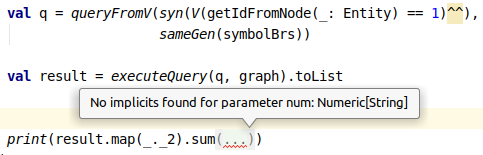
\includegraphics[width=0.48\textwidth]{pictures/image.png}
   \vspace{-0.2cm}
   \caption{Error notification in a query in IntelliJ IDEA}
   \label{fig:types}
\end{figure}
}

\underline{\textbf{IDE Support.}}
By using an IDE to write queries, one can benefit from such features as syntax highlighting, code navigation, autocompletion without any additional effort.
Figure~\ref{fig:autocompletion} shows an example of autocompletion suggestion for a vertex.
{
\setlength{\belowcaptionskip}{-10pt}
\begin{figure}[ht]
    \centering
    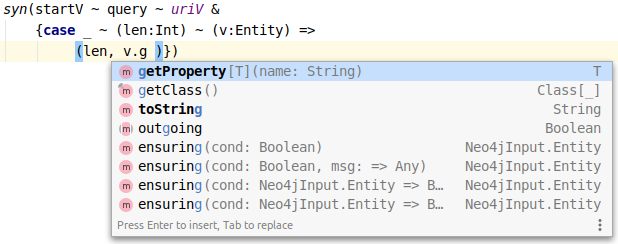
\includegraphics[width=0.48\textwidth]{pictures/image1.png}
    \caption{Query auto-completion in IntelliJ IDEA}
    \label{fig:autocompletion}
\end{figure}
}

In order to test the resulting solution we have implemented the frontend as a plugin using ReSharper SDK, so it can be installed into ReSharper, Rider and InspectCode.
The source code is parsed by internal ReSharper tools and the result is used to produce graphs and meta-information.
The issues found by the backend are shown using code highlighting.

The first analysis which has been implemented is the considered taint tracking analysis.
It is defined just by the PDA constructed in the section 2 translated into the code with some slight modifications which make it possible to process interactions with object fields.
To provide more information about an issue found by this analysis, the higlighting is accompanied by bulbs containing the full path of tainted variable from the source to the sink represented as the sequence of operations.

\subsection{Sample cases}

Let's look closer at properties of the resulting soluiton.
All these properties are illustrated by screenshots taken exactly from the runned Rider IDE with some small relocations of bulbs to make them not to overlap the code.

Firstly, the solution ensures flow sensitivity. I.e. it processes flow of variables passed into methods and returned from them correctly.
Which can be seen at fig~\ref{fig:ReturnsAndBrackets}.
This example illustrates the most common cases of interprocedural data passing.
\textit{Brackets} method gets the data, performs some computations on them and returns the result.
Invocations at lines 37 and 38 shows that the solution can distinguish two data flow paths despite both of them passes through the same method.
So, \textit{e} becomes tainted because \textit{c} is tainted and \textit{f} does not because \textit{d} is clear.
Moreover, the solution can track paths where passes and returns do not form the correct bracket sequence that is shown by method \textit{PostSource} which does not take any parameter and just returns tainted data.

\begin{figure}[h]
	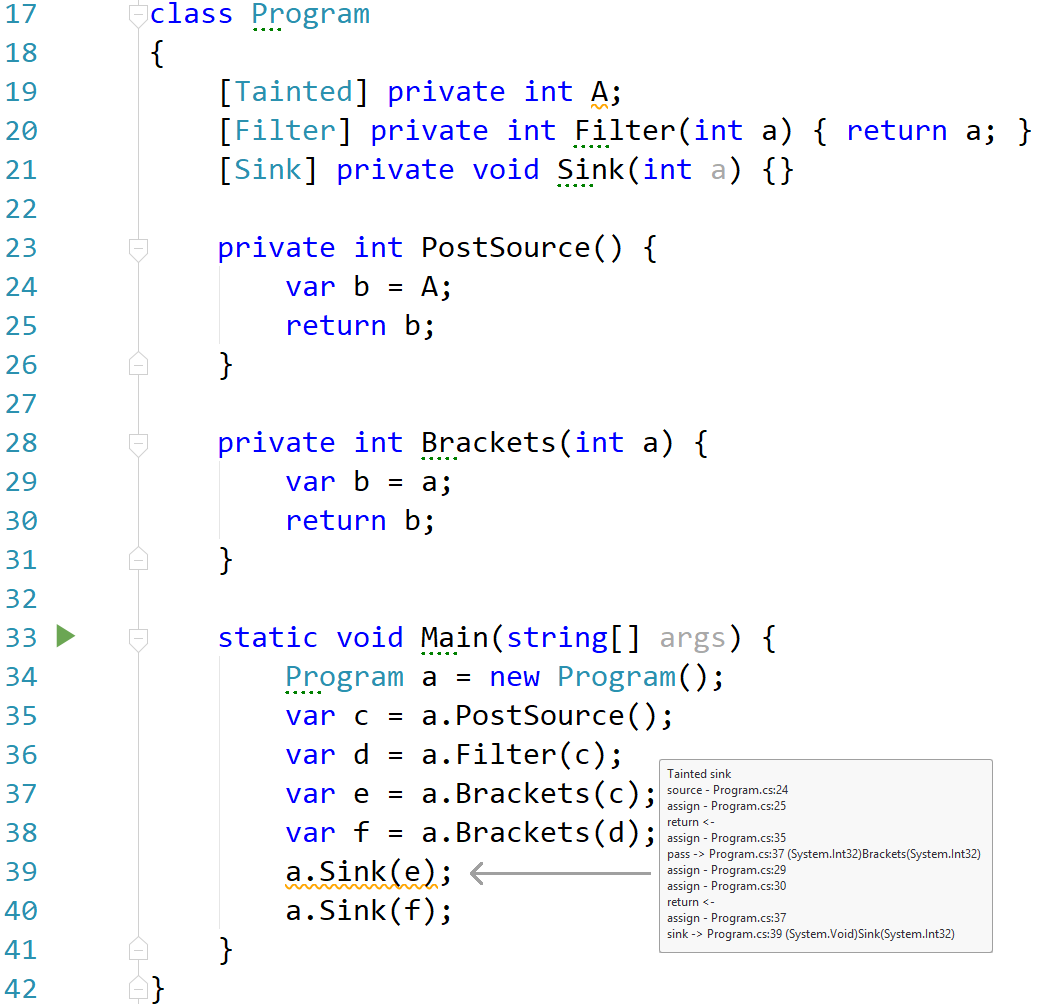
\includegraphics[width=\linewidth]{screenshots/ReturnsAndBrackets.png}
	\caption{Flow sensitivity}
	\label{fig:ReturnsAndBrackets}
\end{figure}

Secondly, the solution has the limited context sensitivity. I.e. it allows to track propagation of objects that are tainted by assigning of some fields inside them both by their own methods and by outer code interacting with their fields directly.
The first case is shown at fig~\ref{fig:ObjectTainting}.
There is the field \textit{B} at the line 18. 
This field can be used widely in the logic of the \textit{Container} class and by this the tainting of this field is considered as the tainting of the whole object.
However, while processing of the method \textit{Store} during the analysis it is hard to decide what the object need to be tainted because in the inner context of \textit{Store} it is just \textit{this} object.
I.e. we must consider the calling context to make such decision.
So, the solution provides this opportunity which is shown by lines 33-36 where the first invocation of \textit{Store} leads to the tainting of object \textit{d} and the second invocation does not taint object \textit{e}.

\begin{figure}[h]
	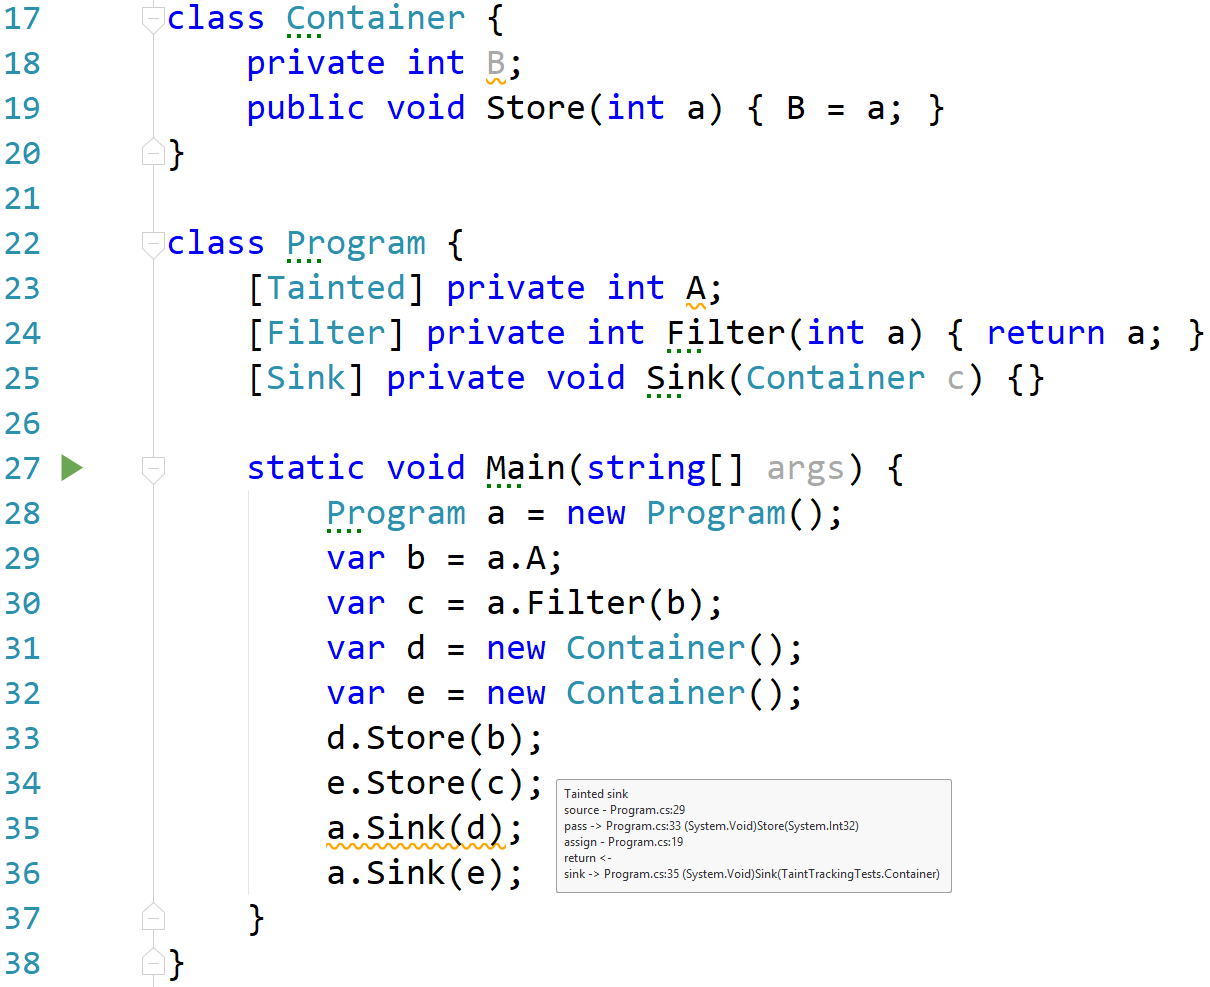
\includegraphics[width=\linewidth]{screenshots/ContextSensitivity.png}
	\caption{Tainting of an object by its own method}
	\label{fig:ObjectTainting}
\end{figure}

Finally, the solution works with any type of recursion and does not fall into infinite cycles.
It can be seen at fig.~\ref{fig:Recursion}.
This snippet contains two mutually recursive methods which pass the data to each other.
The solution checks all possible paths of passing even those which includes cyclic invocations and returns the passed variable to the point corresponding to the initial invocation.

\begin{figure}[h]
	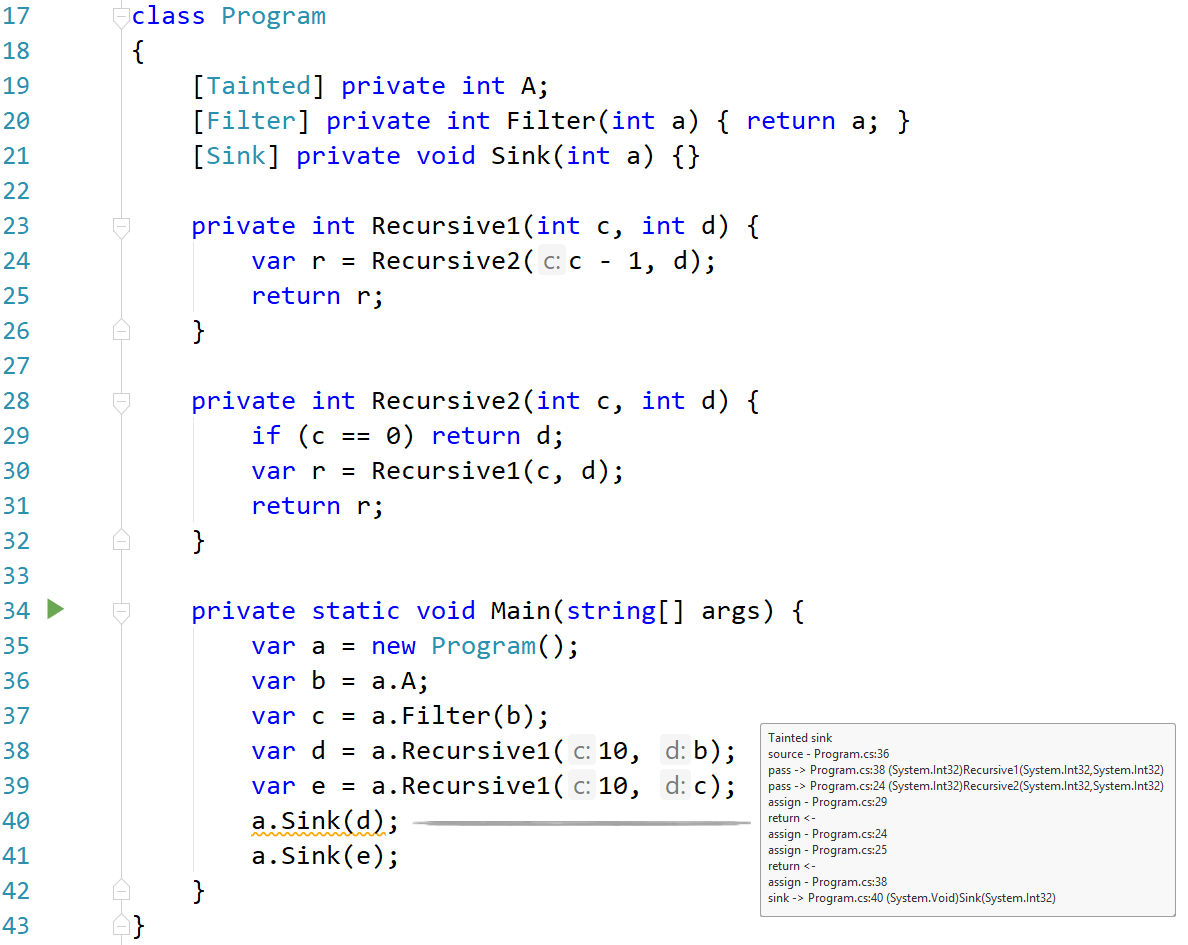
\includegraphics[width=\linewidth]{screenshots/Recursion.png}
	\caption{Recursive methods processing}
	\label{fig:Recursion}
\end{figure}

\subsection{Performance}

It is also necessary to measure the performance of the resulting solution.
Because the implemented taint tracking analysis forces to mark all participating entities manually, it is difficult to perform it on some large project.
However, there is another intermediate analysis which is runned before any other one to collect some information required by resolver.
In particular, it tracks propagation of all variables to discover all possible concrete types of each variable.
So, it involves each variable and each method in the whole program and thus the time and space required for execution of this analysis may be consistent estimation of the efficiency of the solution.

The code base that has been chosen as a source of data is the full solution of the Mono project.
(TODO: ADD SYSTEM CONFIGURATION).
The results is shown in the table~\ref{tab:Performance}.

\begin{table}[h]
	\begin{tabular}{|l|l|l|l|l|}
	\hline
		Project & Classes & Methods & \begin{tabular}[c]{@{}l@{}}Execution \\ time (s)\end{tabular} & \begin{tabular}[c]{@{}l@{}}Allocated \\ memory (GB)\end{tabular} \\ \hline
		Mono & 21013 & 192745 & $21\pm 0.5$ & $\sim 4.2$ \\ \hline
	\end{tabular}
	\caption{Performance}
	\label{tab:Performance}
\end{table}

\section{Conclusion}

We propose and implement in C\# programming language the generic framework for interprocedural static code analysis implementation.
This framework allows one to implement arbitrary interprocedural analysis in terms of CFL-reachability.
By using the proposed framework, we implement a plugin upon ReSharper infrastructure which provides simple taint analysis and demonstrate that our solution can handle important real-world cases.
Also we show that the proposed framework can be used for real-world solutions analysis.

One of the directions for future work is a creation of analysis and its evaluation on real-world projects.
By this way, we want to get information which helps to improve the usability of our framework: tune performance, improve API, etc.
Also we should improve documentation and create more examples of usage.

Another direction is a practical evaluation of automatic fix location prediction by using minimum cuts method~\cite{10.1007/978-3-319-63390-9_27}.

Also we want to compare the proposed approach with other generic CFL-reachability based approaches for interprocedural code analysis cretion. For example, fith generation-based approach~\cite{LPAR-21:Cauliflower_Solver_Generator_for}, which idea is similar to parser generators.

%%
%% The acknowledgments section is defined using the "acks" environment
%% (and NOT an unnumbered section). This ensures the proper
%% identification of the section in the article metadata, and the
%% consistent spelling of the heading.
\begin{acks}
To Robert, for the bagels and explaining CMYK and color spaces.
\end{acks}

%%
%% The next two lines define the bibliography style to be used, and
%% the bibliography file.
\bibliographystyle{ACM-Reference-Format}
\bibliography{Combinators_for_single_source_CFPQ}


\end{document}
\endinput
%%
%% End of file `sample-sigconf.tex'.
